\chapter{Next\_Comput}

\section{Purpose}
%
The aim of this case is to test a computation that follows another one. We start from a calculated state at a time and we simulate some new time step.
%
\section{Description of the problem}
%
The simulation is the same as the shoal test case so one will read that test case for physical description. We start here from a shoal simulation until time 600s. The result of this previous simulation is inside the file indicated by the keyword {\it PREVIOUS COMPUTATION FILE} ({\it FICHIER DU CALCUL PRECEDENT} in french). This file has been created by adding the keyword  {\it GLOBAL RESULT FILE} ({\it FICHIER DES RESULTATS GLOBAUX} in french) in the shoal steering case.
We simulate for 600 other seconds. We can compare the result to the one obtained by shoal test case with 1200 seconds of simulation.

\section{Results}
After 600 s, the difference with the full shoal simulation is null.
\begin{figure} [!h]
\centering
\includegraphicsmaybe{[width=0.85\textwidth]}{../img/results.png}
%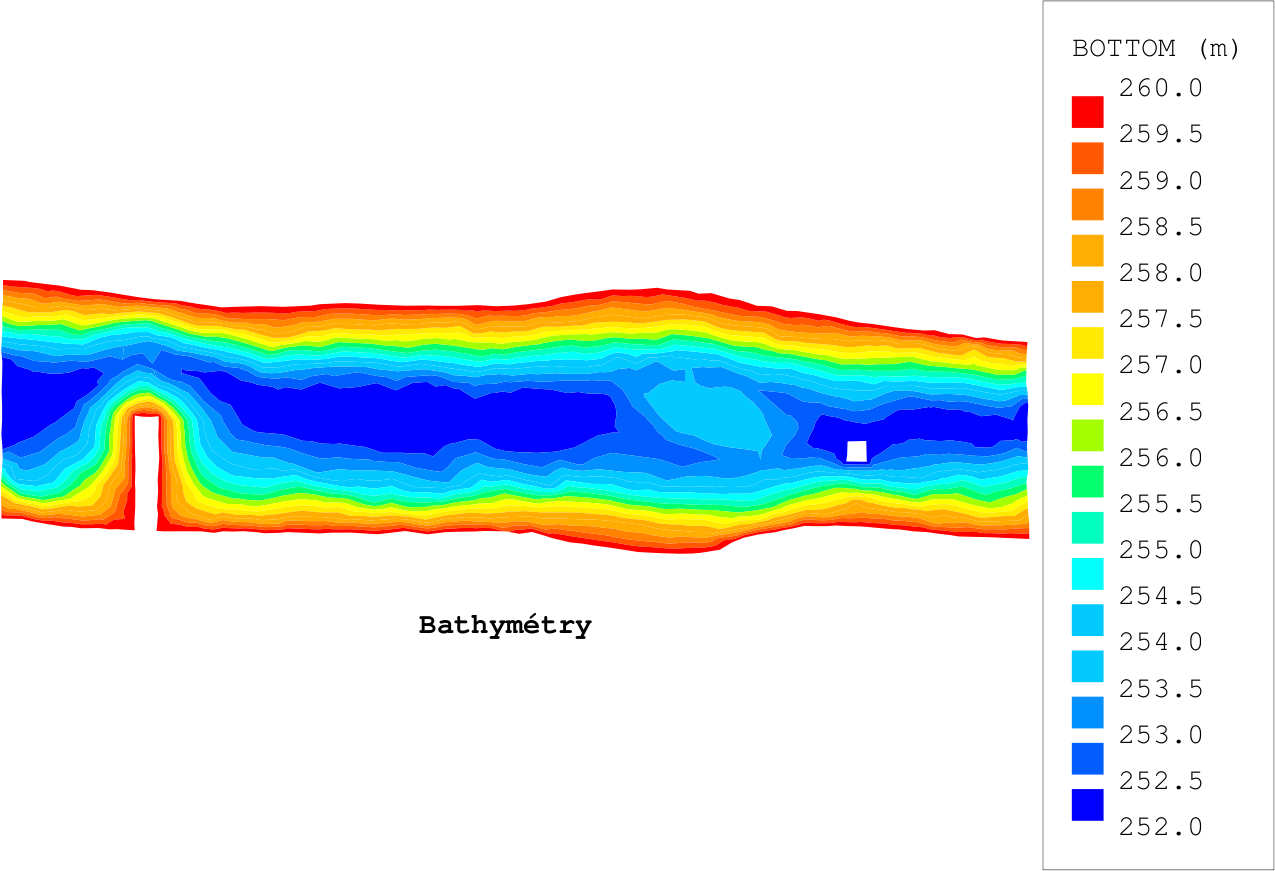
\includegraphics{bathy.png}
 \caption{Wave heigth HM0}
\label{resnextcomp}
\end{figure}
